\documentclass{beamer}
\usepackage[utf8]{inputenc}
\usepackage{mathtools}
\usepackage{bm}
\usepackage{circuitikz}
\usepackage{tcolorbox}
\usepackage{forest}
\usepackage{minted}

\usetheme{Dresden}
\setbeamersize{text margin left=.3cm,text margin right=.5cm}
\setbeamertemplate{itemize items}[square]

\title{Toy SSVF}
\author{Lucio Derin}
\date{12/12/2022}
\titlegraphic{
\includegraphics[width=3cm]{../screenshots/logo.png}}
\setbeamercovered{transparent}
\setbeamertemplate{footline}[frame number]
\setbeamertemplate{headline}{}
%1 titolo
\begin{document}
\begin{frame}[plain]    
    \maketitle
\end{frame}

%2 Project Description
\begin{frame}
    \frametitle{Project description}
    \only<1>{
        \begin{columns}
            \begin{column}{0.35\textwidth}
                \begin{center}
                    SSVF:
                    ~\\
                    ~\\
                    \begin{forest}
                        [Jet[Vertex Finding[Vertex Fitting]]]
                    \end{forest}
                \end{center}
            \end{column}
            \begin{column}{0.65\textwidth}
                \begin{center}
                    GN1:
                    ~\\
                    ~\\
                    \begin{forest}
                        [Jet
                            [Vertex Finding,name=vf
                                [p1,phantom]
                            ]
                            [b-tagging,name=bt
                                [p2,phantom[Loss,name=shared]]
                            ]
                            [Tracks' origins,name=to[p3,phantom]]
                        ]
                        \draw (vf) -- (shared);
                        \draw (bt) -- (shared);
                        \draw (to) -- (shared);
                        \end{forest}
                \end{center}
            \end{column}
        \end{columns}
    }
    \only<2>{
        \begin{center}
            \begin{forest}
                [p1,phantom
                [Jet[Vertex Finding,name=vf1[Vertex Fitting,name=vfit]]]
                [Jet
                            [Vertex Finding,name=vf
                                [p1,phantom]
                            ]
                            [b-tagging,name=bt
                                [p2,phantom[Loss,name=shared]]
                            ]
                            [Tracks' origins,name=to[p3,phantom]]
                ]
                ]
                \draw (vf) -- (shared);
                \draw (bt) -- (shared);
                \draw (to) -- (shared);
                \draw[very thick,red] (vf1) -- (vf);
                \end{forest}
        \end{center}
    }
    \only<3>{
        \begin{center}
            \begin{forest}
                [p1,phantom
                [Jet[Vertex Finding,name=vf1[Vertex Fitting,name=vfit]]]
                [Jet
                            [Vertex Finding,name=vf
                                [p1,phantom]
                            ]
                            [b-tagging,name=bt
                                [p2,phantom[Loss,name=shared]]
                            ]
                            [Tracks' origins,name=to[p3,phantom]]
                ]
                ]
                \draw (vf) -- (shared);
                \draw (bt) -- (shared);
                \draw (to) -- (shared);
                \draw[very thick,red] (vf1) -- (vf);
                \draw[very thick,red] (vfit) -- (shared);
                \end{forest}
        \end{center}
    }
    
\end{frame}

%3 Step 0: vertex finding
\begin{frame}[fragile]
    \frametitle{Step 0: understanding vertex finding (pseudo-code)}
    \definecolor{bg}{rgb}{0.95,0.95,0.95}
    \begin{minted}[bgcolor=bg]{python}
# List of coupled tracks (two-tracks vertex approximation)
couples = []
indices = [i for i in range(len(tracks))]
# While there are tracks to be coupled
while len(tracks)>1:
    # Select the track to be coupled
    i,t = indices.pop(0),tracks.pop(0)
    #selecting the closest track
    j = argmin(distances)
    # if tracks are close enough, couple them
    if distances[j] < threshold:
        tc = tracks.pop(j)
        indices.pop(j)
        couples.append([t,tc])
return couples
    \end{minted}
\end{frame}

%4 Step 0: vertex fitting
\begin{frame}[fragile]
    \frametitle{Step 0: understanding vertex fitting (pseudo-code)}
    \definecolor{bg}{rgb}{0.95,0.95,0.95}
    \begin{minted}[bgcolor=bg]{python}
# fitting loop
while True:
    # Find the SV that minimizes the chi2
    # from the current selected tracks
    SVfitted = min(chi2(tracks))
    # If chi2 is good enough, break
    if chi2 < threshold:
        break
    # Else, reject the worst track
    tracks.pop(argmax(chi2s))
    # If there are less than 2 tracks,
    # no vertex has been found
    if len(tracks)<2:
        return None
return SVfitted
    \end{minted}
\end{frame}

%5 Toy model
\begin{frame}
    \frametitle{Testing the algorithm: Toy Jets}
    \begin{center}
        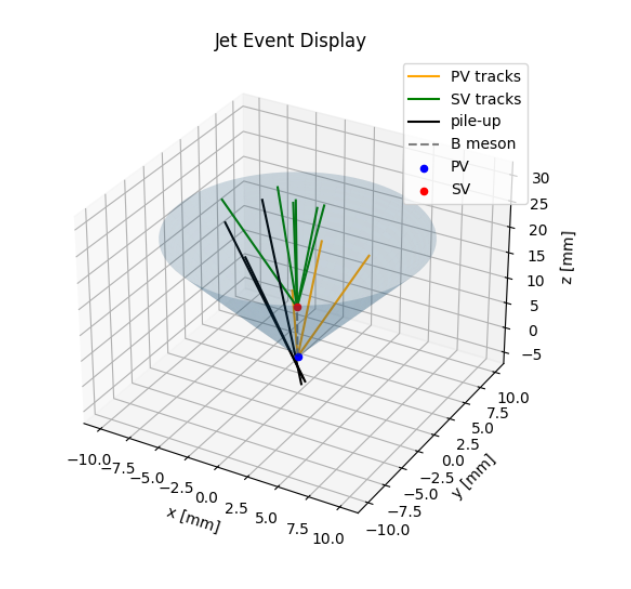
\includegraphics[width=0.8\textwidth]{../screenshots/eventDisplay.png}
    \end{center}
\end{frame}

%6 SSVF
\begin{frame}
    \frametitle{Testing the algorithm: SSVF on toy Jets}
    \begin{center}
        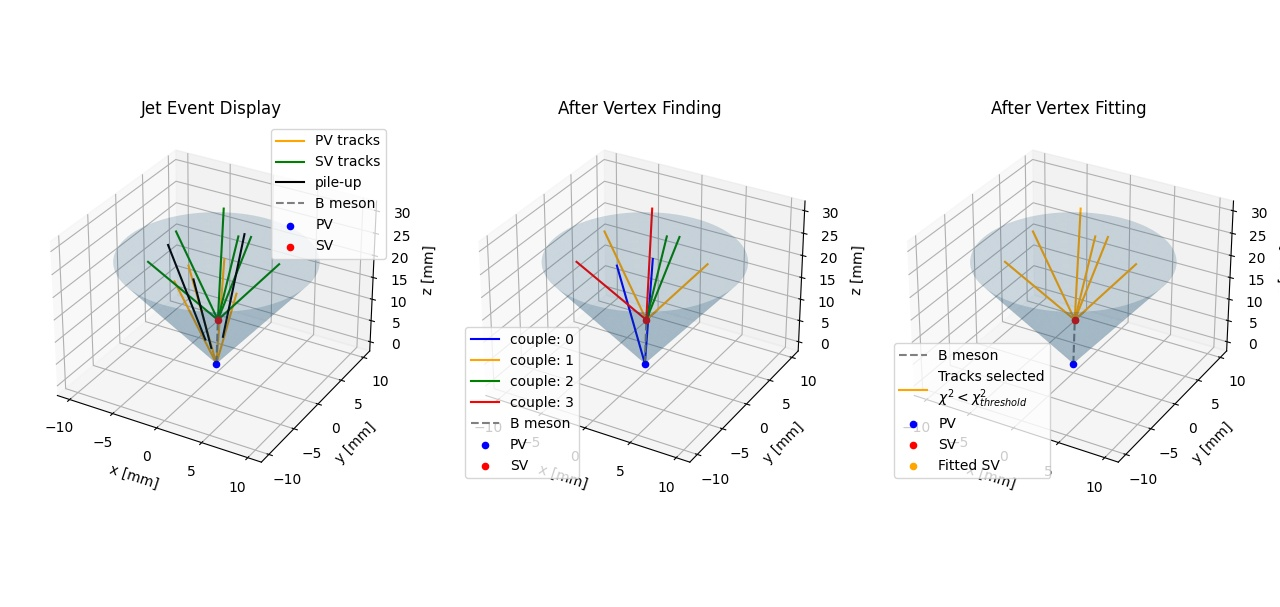
\includegraphics[width=\textwidth]{../screenshots/jetEventCone2.jpg}
    \end{center}
\end{frame}

%7 SSVF errors
\begin{frame}
    \frametitle{Testing the algorithm: SSVF errors on 100 Jets}
    \only<1>{
        \begin{center}
            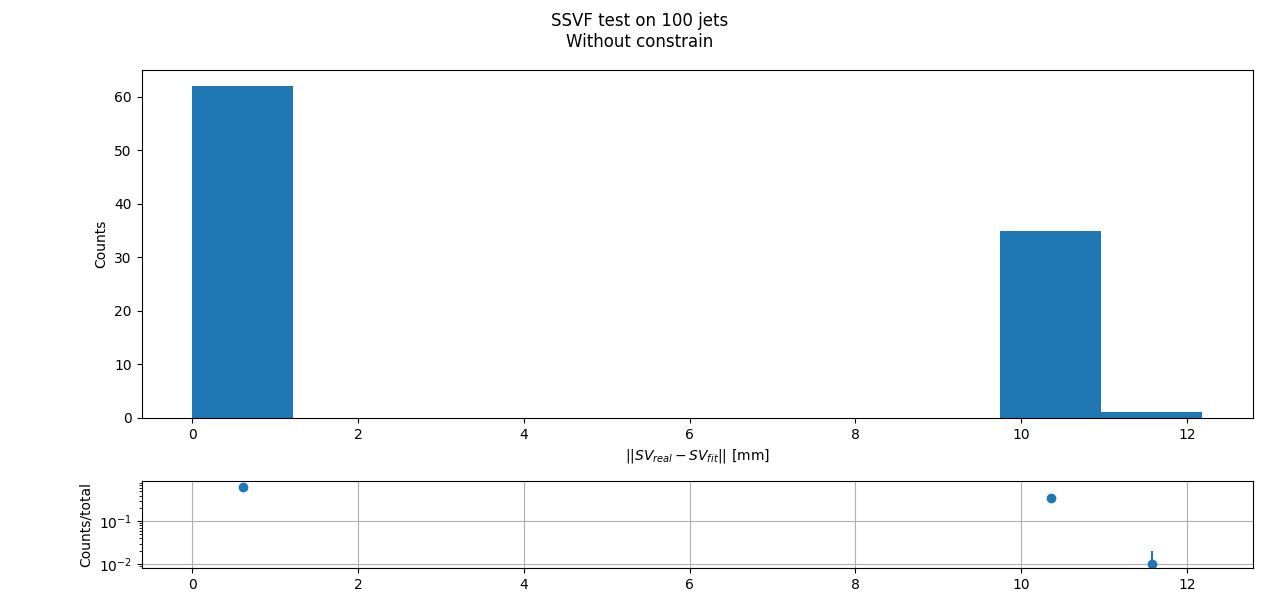
\includegraphics[width=\textwidth]{../screenshots/ssvfErrors.png}
        \end{center}
    }
    \only<2>{
        \begin{center}
            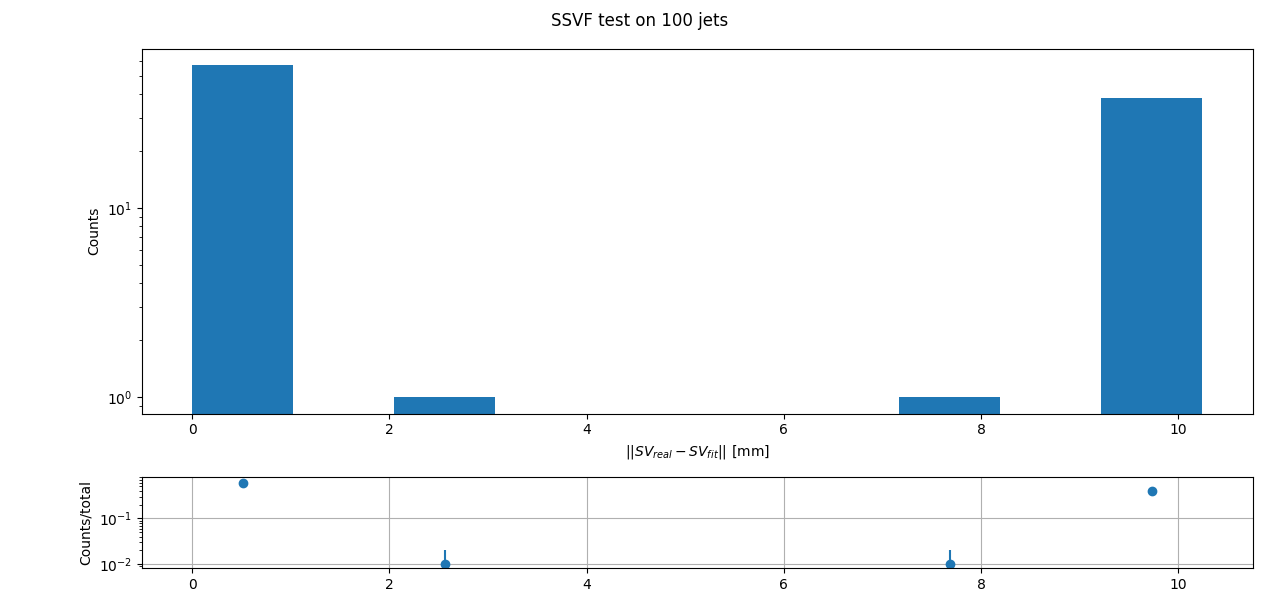
\includegraphics[width=\textwidth]{../screenshots/ssvfErrorsLog.png}
        \end{center}
    }
\end{frame}

\begin{frame}
    \frametitle{Error 1: fit converges to PV}
    \begin{center}
        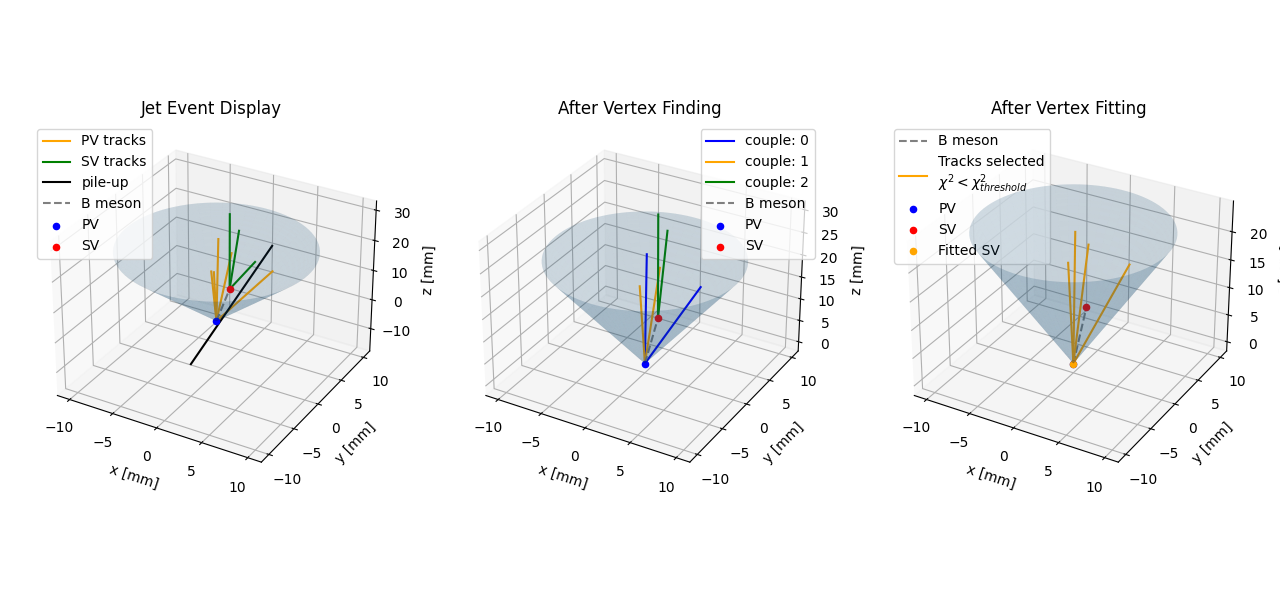
\includegraphics[width=\textwidth]{../screenshots/misclassifiedPV.png}
    \end{center} 
\end{frame}

\begin{frame}
    \frametitle{Error 2: tracks from PV are not rejected}
    \begin{center}
        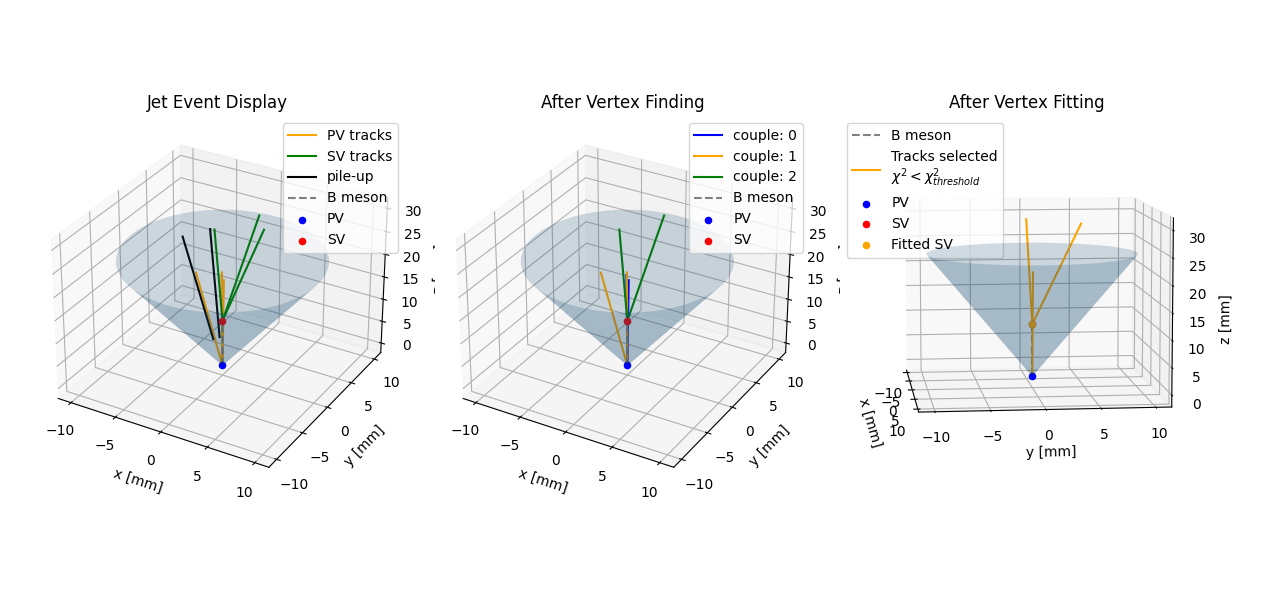
\includegraphics[width=\textwidth]{../screenshots/noise1.png}
    \end{center} 
\end{frame}

\begin{frame}
    \frametitle{Alternative algorithm: clustering-based vertex finding}
    \only<1-2>{
        SSVF:
        \begin{itemize}
            \item<1-2> Needs PV's tracks rejection to avoid convergence to PV;
            \item<2> $O(N^2)$
        \end{itemize}
    }
    \only<3->{
        C-SSVF based on K-Means clustering:
        \begin{itemize}
            \item<3-> Automatically clusters together only high IP tracks from SV;
            \item<4> LLoyd implementation: $O(tkNd) \implies O(N)$
        \end{itemize}
    }
    \only<4>{
        $$\min\limits_{m_i \in \mathbb{R}^D}\sum\limits_{i=1}^n\min\limits_{j=1,K} |x_i-m_j|^2$$
    }
\end{frame}

\begin{frame}
    \frametitle{Culstering based vertex finding}
    \only<1>{
        \begin{center}
            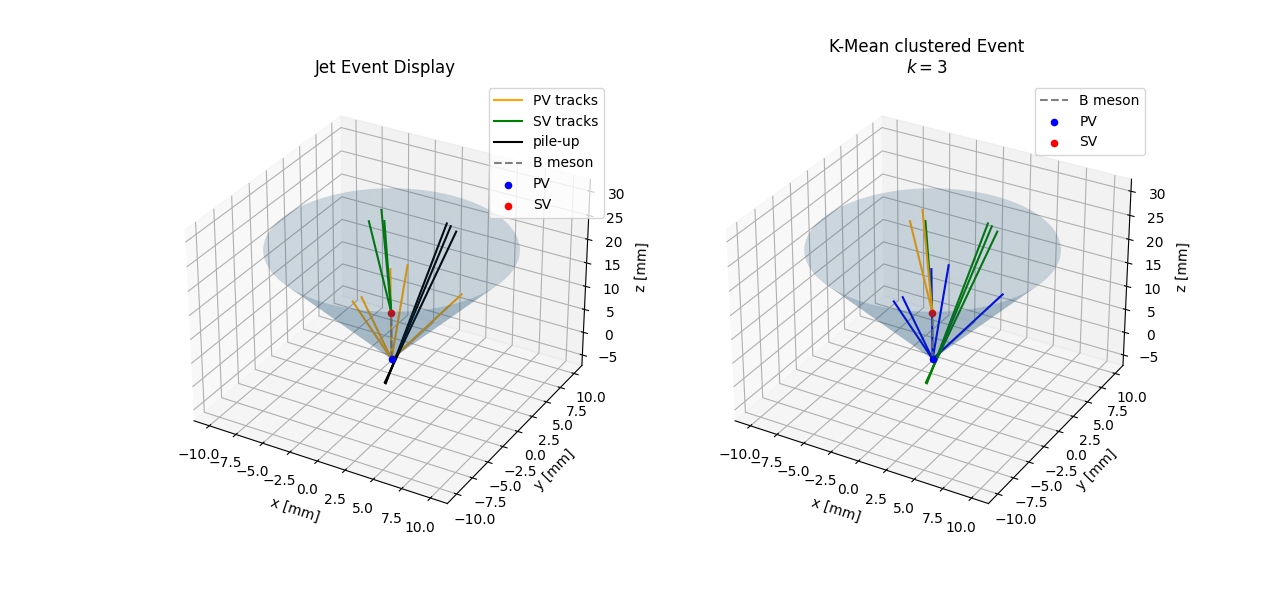
\includegraphics[width=\textwidth]{../screenshots/clustering.png}
        \end{center} 
    }
    \only<2>{
        \begin{center}
            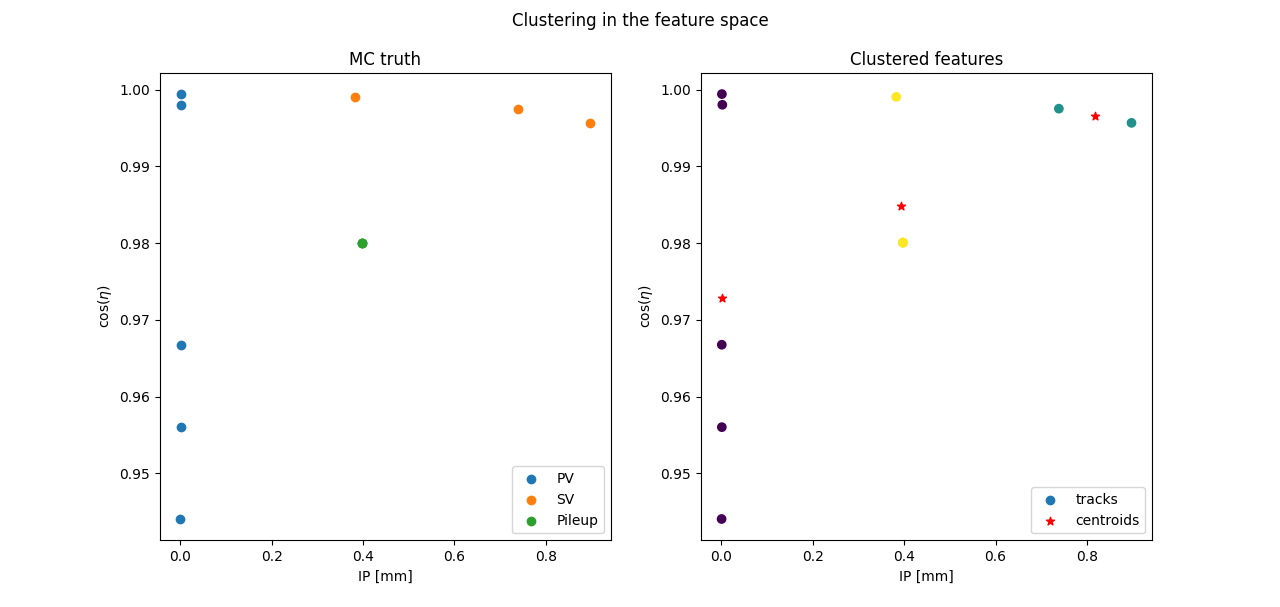
\includegraphics[width=\textwidth]{../screenshots/clusteringFeatures.png}
        \end{center} 
    }
\end{frame}

\begin{frame}
    \frametitle{Testing the algorithm: C-SSVF errors on 100 Jets}
    \begin{center}
        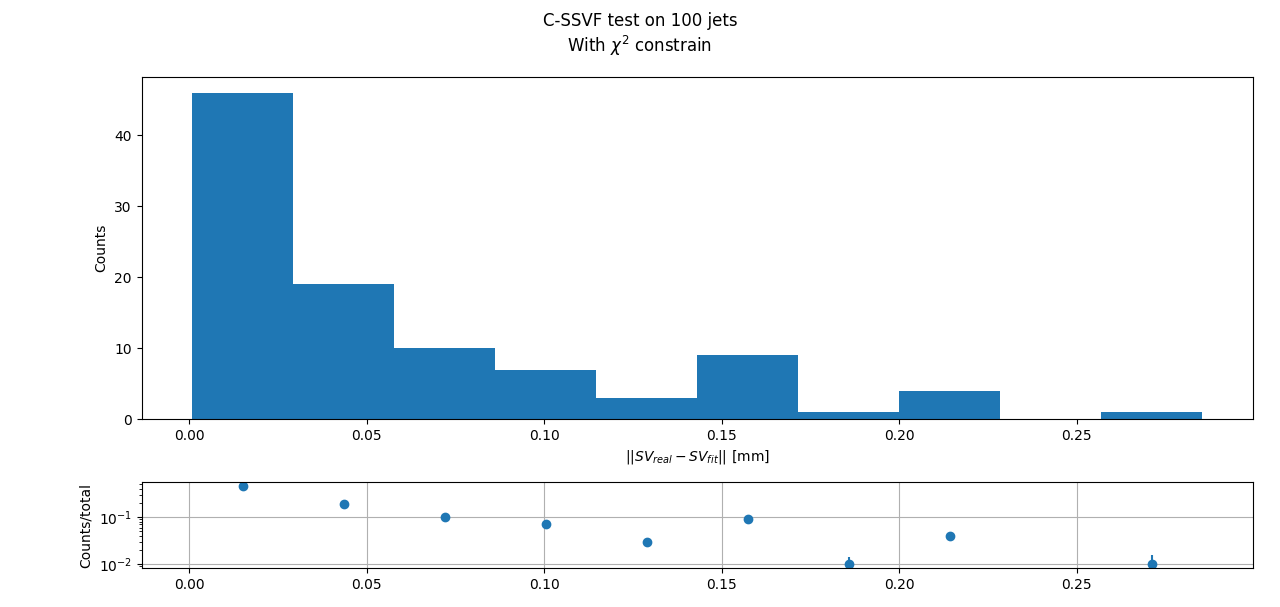
\includegraphics[width=\textwidth]{../screenshots/cssvf.png}
    \end{center}
\end{frame}
\begin{frame}
    \frametitle{SSVF vs C-SSVF}
    \begin{center}
        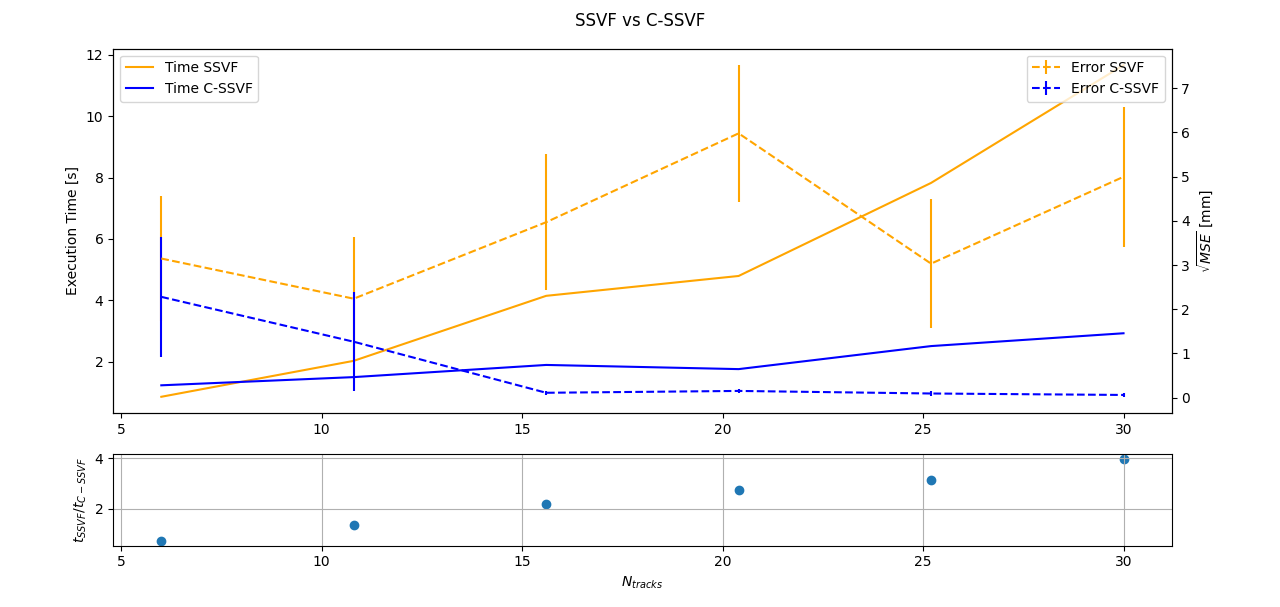
\includegraphics[width=\textwidth]{../screenshots/ssvfVScssvf.png}
    \end{center}
\end{frame}

\begin{frame}
    \frametitle{C-SSVF in dense jets}
    \only<1>{
        \begin{center}
            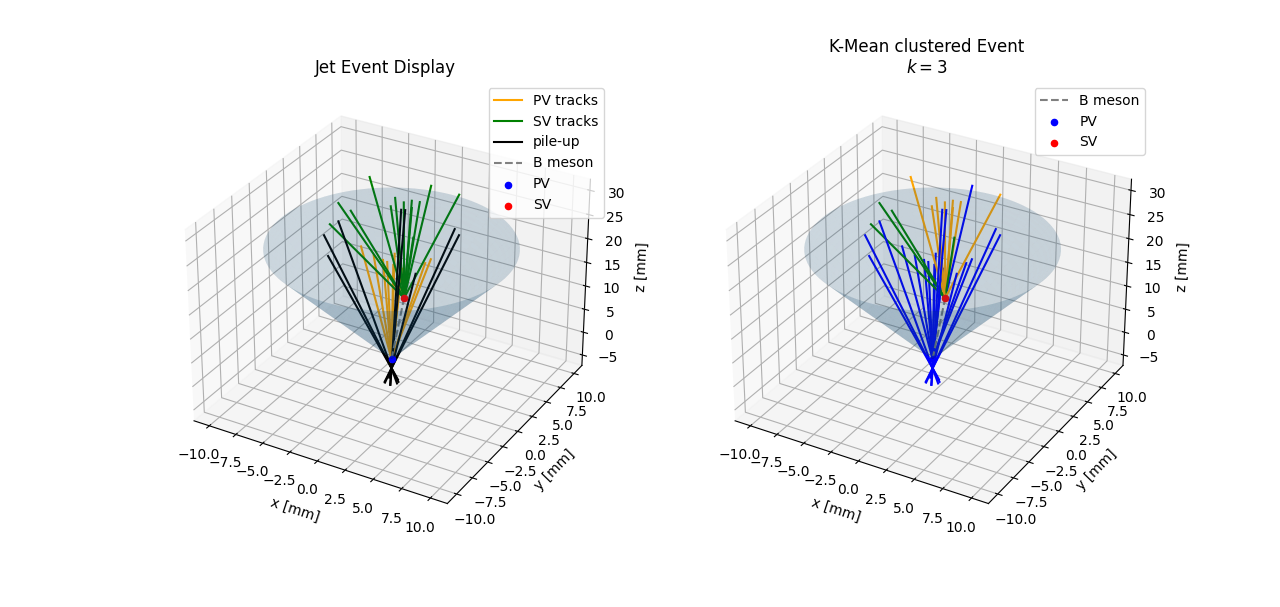
\includegraphics[width=\textwidth]{../screenshots/clusteringHighLum.png}
        \end{center}
    }
    \only<2>{
        \begin{center}
            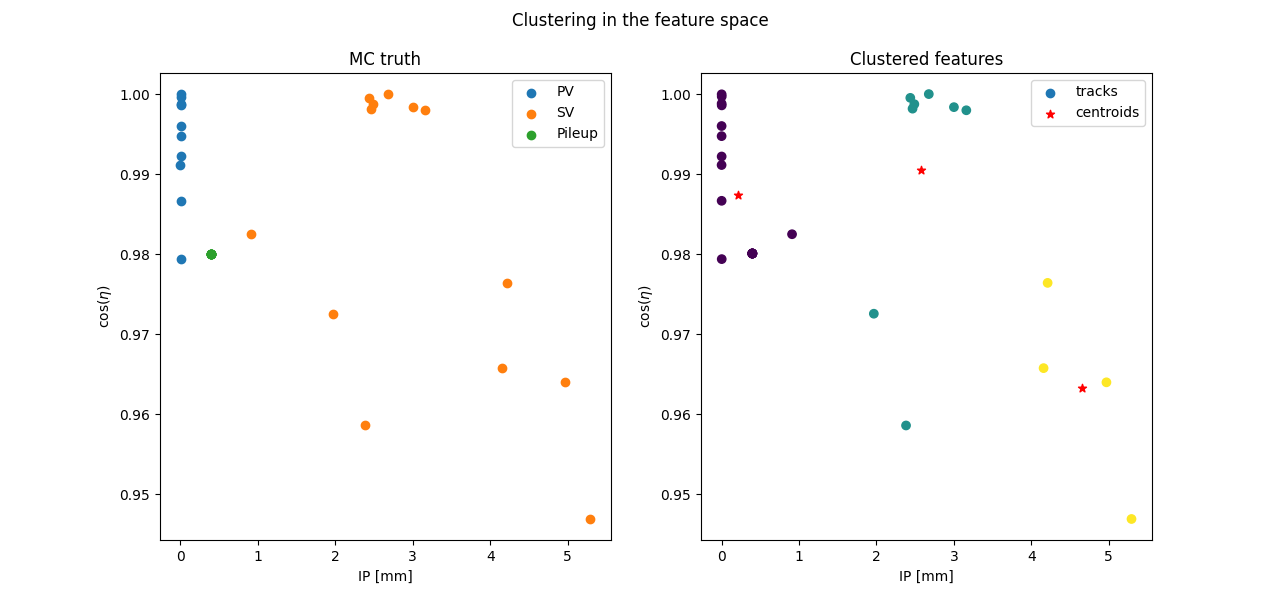
\includegraphics[width=\textwidth]{../screenshots/clusteringFeaturesHighLum.png}
        \end{center}
    }
\end{frame}

\begin{frame}
    \frametitle{Next up}
    \begin{itemize}
        \item<1-> Display real Jets;
        \item<2-> Apply SSVF to real Jets;
        \item<3-> Repeat all previous analysis on real Jets;
        \item<4-> ... 
    \end{itemize}
\end{frame}
\end{document}